%! TEX root = ../main.tex
\documentclass[../main]{subfiles}

% ローカル下書き用
% \documentclass{supernova_pre}
% このクラスの中に大体のパッケージは入ってるので基本何でもかけるはず
% 追加したいパッケージがあればここに記入
\usepackage{multicol}
\usepackage{caption}

\begin{document}
\chapter{2024年度 沖縄夏合宿} % タイトル
\rightline{1年 新田 章仁、戸倉 翔大} % 学年と名前(ハンドルネームでも可)
\section{概要}
2024年9月26日から29日にかけて天文部の夏合宿が沖縄県で行われました。ここでは、合宿の様子を紹介します。
\subsection{行先}
沖縄県 本島 / 座間味島
\subsection{日程}
2024年9月26日(木) ~ 9月29日(日)
\begin{figure}[htbp]
    \centering
    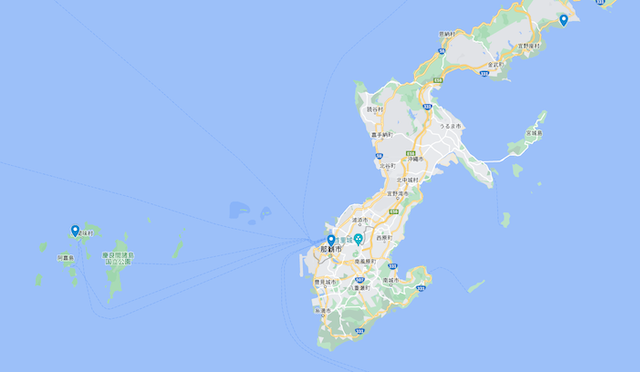
\includegraphics[width=14cm]{sections/Nitta_Tokura/figure/map_okinawa.png}
    \caption{大まかな地図}
\end{figure}
\subsection{宿泊施設}
ゲストハウス海風、阿真コテージ
\subsection{参加者}
1年~3年生 計19名
\section{行程概要}
% \begin{wrapfigure}{r}[0pt]{0.5\textwidth}
%     \centering
%       \includegraphics[width=6cm]{figure/IMG_9295.JPG}
%     \caption{水と緑のふれあい館}
%     \label{fig:arc}
% \end{wrapfigure}
\begin{multicols}{2}
\begin{description}
    \item 1日目
    \begin{description}
        \item 10:30 部室集合
        \item 11:40 調布駅
        \item 13:50 成田空港
        \item 昼食
        \item 16:00 成田空港 発
        \item 19:00 那覇空港 着
        \item 那覇空港で夕食
        \item 20:20 那覇空港 発
        \item 20:55 ゲストハウス 海風 着
        \item 21:50 ホテル 発
        \item 23:00 シーグラスビーチ 着
        \item 23:10 天体観測
    \end{description}
    \item 2日目
    \begin{description}
        \item  3:00 ホテル 着
        \item (就寝・各自自由行動)
        \item 16:00 泊港 発
        \item 17:10 座間味港 着
        \item 17:45 阿真コテージ 着
        \item (夕食・就寝)
        \item 
        \item 
        \item 
        \item 
    \end{description}
\end{description} 
\end{multicols}
\begin{multicols}{2}
\begin{description}
    \item 3日目
    \begin{description}
        \item 自由行動
        \item 12:00 昼食
        \item 自由行動
        \item 18:00 夕食
        \item 21:00 天体観測
        \item
        \item 
        \item 
    \end{description}
    \item 4日目
    \begin{description}
        \item  9:00 コテージ 発
        \item 10:00 座間味港 発
        \item 11:10 泊港 着
        \item 自由行動
        \item 18:25 那覇空港 発
        \item 21:00 成田空港 着
        \item 解散
    \end{description}
\end{description} 
\end{multicols}
  
1年生は新歓合宿に引き続き、2回目の合宿でした。また、初めて合宿に参加する部員も多くみんなワクワクしていました!
\\

\section{当日の様子}
\subsection{1日目}
1日目は多くの時間を移動に費やし、沖縄には夜に着きました。\\
\begin{figure}[H]
  \begin{minipage}[b]{0.48\columnwidth}
    \centering
    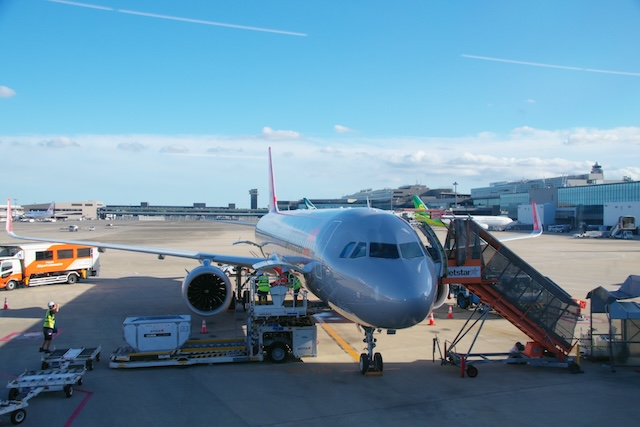
\includegraphics[width=\columnwidth]{sections/Nitta_Tokura/figure/hikouki.jpg}
  \end{minipage}
  \hspace{0.04\columnwidth} % ここで隙間作成
  \begin{minipage}[b]{0.48\columnwidth}
    \caption{\\
    沖縄までの飛行機\\
    学生の味方。機内では多くの部員が寝ていました。
    }
  \end{minipage}
\end{figure}

\begin{figure}[H]
  \begin{minipage}[b]{0.48\columnwidth}
    \caption{\\
    ソーキそば\\
    ジューシーなソーキと太めでコシのある麺がマッチしていて、とてもおいしかったです!!
    }
  \end{minipage}
  \hspace{0.04\columnwidth} % ここで隙間作成
  \begin{minipage}[b]{0.48\columnwidth}
    \centering
    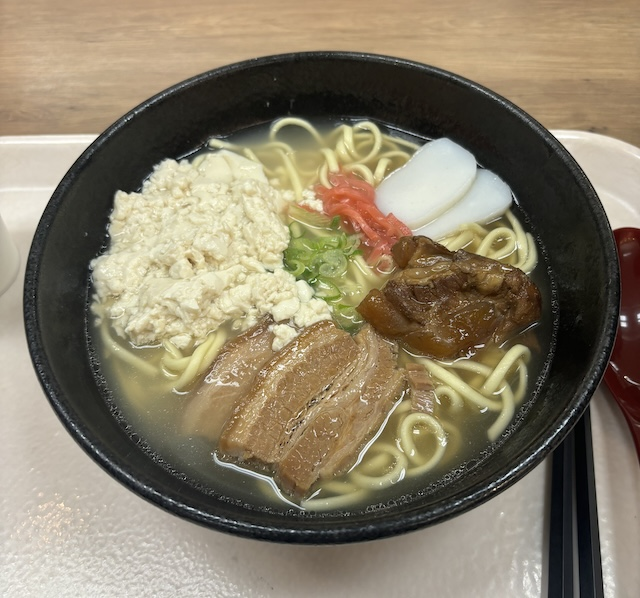
\includegraphics[width=0.7\columnwidth]{sections/Nitta_Tokura/figure/okinawasoba.jpg}
  \end{minipage}
\end{figure}

合宿期間を通して1日目の夜が一番良い天候と分かったので、急遽名護市のシーグラスビーチまでレンタカーで行きました。視界が開けた場所でとても撮影がしやすい場所で、満点の星空が眺められました!
\begin{figure}[H]
  \begin{minipage}[b]{0.48\columnwidth}
    \centering
    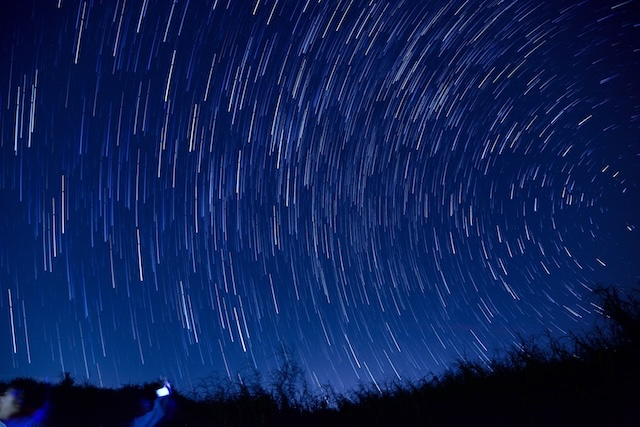
\includegraphics[width=\columnwidth]{sections/Nitta_Tokura/figure/hosi_suttakku_1nitime.jpg}
  \end{minipage}
  \hspace{0.04\columnwidth} % ここで隙間作成
  \begin{minipage}[b]{0.48\columnwidth}
    \caption{\\
    シーグラスビーチで撮影した写真
    }
  \end{minipage}
\end{figure}

\begin{figure}[H]
  \begin{minipage}[b]{0.48\columnwidth}
    \caption{\\
    シーグラスビーチで撮影した写真\\
    南の方は曇っていましたが、他の方角は雲がほとんどなくよく星が見えました。
    }
  \end{minipage}\hspace{0.04\columnwidth}\begin{minipage}[b]{0.48\columnwidth}
    \centering
    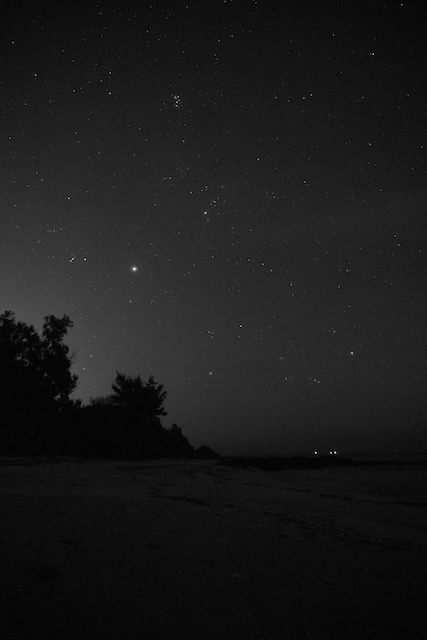
\includegraphics[width=0.7\columnwidth]{sections/Nitta_Tokura/figure/1nitimeyoru.jpg}
  \end{minipage}
\end{figure}


\subsection{2日目}
2日目の昼間は自由行動の時間だったので、各々いろんなところに行きました。部員が行った場所を紹介します。\\
\subsubsection*{・首里城組}
\begin{figure}[H]
  \begin{minipage}[b]{0.48\columnwidth}
    \centering
    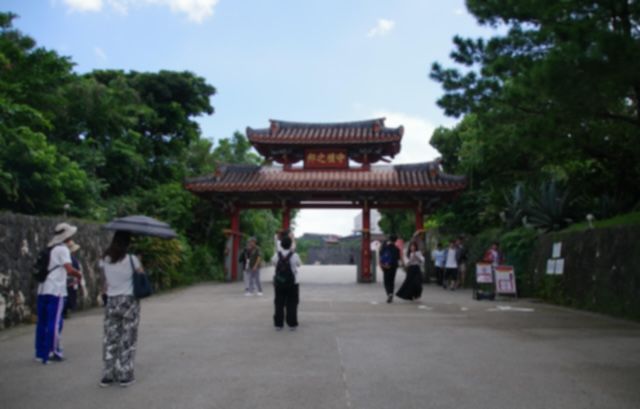
\includegraphics[width=\columnwidth]{sections/Nitta_Tokura/figure/syureimon_bokasi.jpg}
  \end{minipage}
  \hspace{0.04\columnwidth} % ここで隙間作成
  \begin{minipage}[b]{0.48\columnwidth}
    \caption{\\
    守礼門\\
    2000円札にも載っている守礼門は大きかったです。
    }
  \end{minipage}
\end{figure}

\begin{figure}[H]
  \begin{minipage}[b]{0.48\columnwidth}
    \caption{\\
    首里城\\
    2019年に火事で正殿は焼け落ちたので、合宿で行った時には首里城再建に向けて工事をしていました。首里城ではハイビスカスが咲いているところも見れました。
    }
  \end{minipage}
  \hspace{0.04\columnwidth} % ここで隙間作成
  \begin{minipage}[b]{0.48\columnwidth}
    \centering
    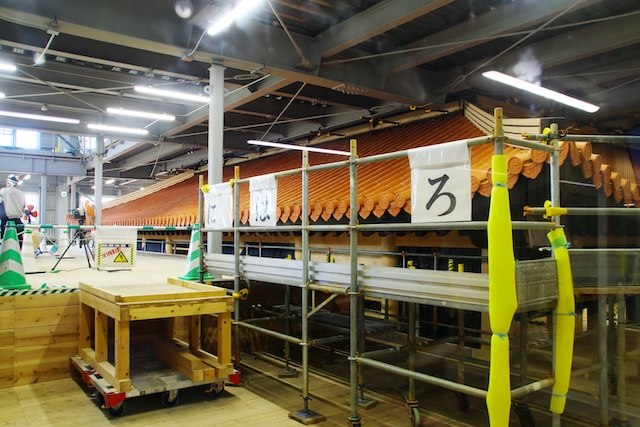
\includegraphics[width=\columnwidth]{sections/Nitta_Tokura/figure/kouzityuu_syurizyou.jpg}
  \end{minipage}
\end{figure}

\begin{figure}[H]
  \begin{minipage}[b]{0.48\columnwidth}
    \centering
    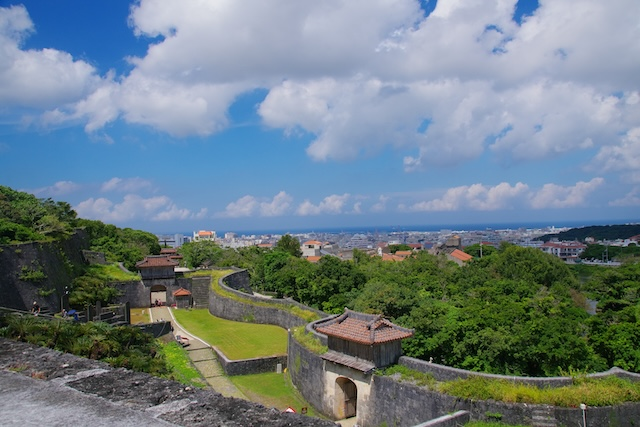
\includegraphics[width=\columnwidth]{sections/Nitta_Tokura/figure/view_syurizyou.jpg}
  \end{minipage}
  \hspace{0.04\columnwidth} % ここで隙間作成
  \begin{minipage}[b]{0.48\columnwidth}
    \caption{\\
    首里城からの眺め\\
    首里城からの眺めはよく、遠くに海も見えました。
    }
  \end{minipage}
\end{figure}

\begin{figure}[H]
  \begin{minipage}[b]{0.48\columnwidth}
    \caption{\\
    昼食\\
    沖縄で有名な料理店であるステーキハウス88でご飯を食べました。
    }
  \end{minipage}
  \hspace{0.04\columnwidth} % ここで隙間作成
  \begin{minipage}[b]{0.48\columnwidth}
    \centering
    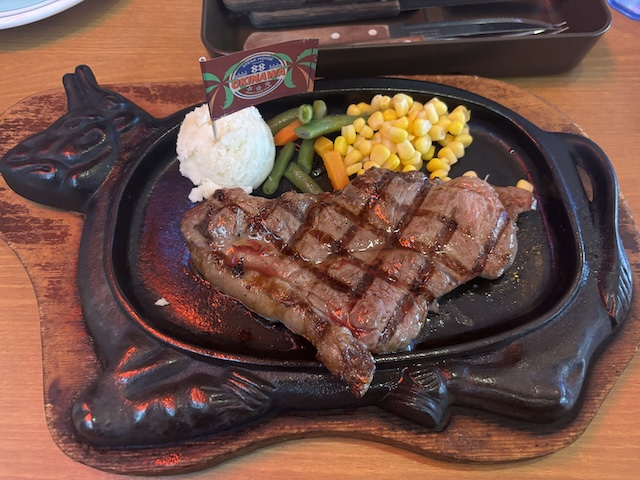
\includegraphics[width=\columnwidth]{sections/Nitta_Tokura/figure/steak88.jpeg}
  \end{minipage}
\end{figure}

\subsubsection*{・美ら海水族館組}
\begin{figure}[H]
  \begin{minipage}[b]{0.48\columnwidth}
    \centering
    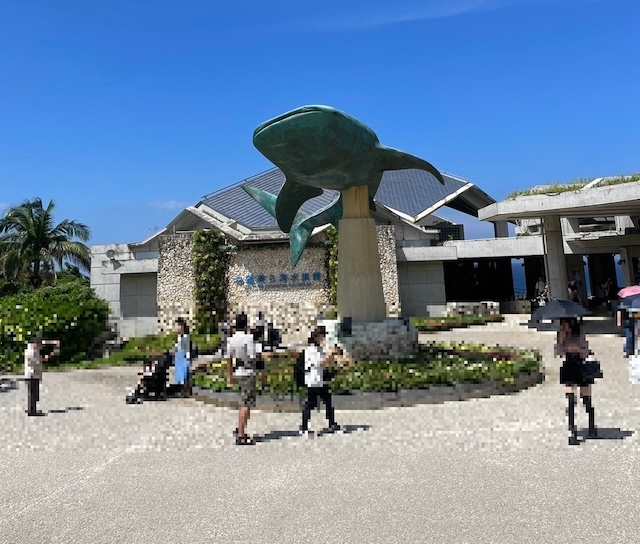
\includegraphics[width=0.8\columnwidth]{sections/Nitta_Tokura/figure/tyuraumi_entrance.jpg}
  \end{minipage}
  \hspace{0.04\columnwidth} % ここで隙間作成
  \begin{minipage}[b]{0.48\columnwidth}
    \caption{\\
    水族館入口\\
    美ら海水族館で有名なジンベイザメの大きな像がいました。
    }
  \end{minipage}
\end{figure}

\begin{figure}[H]
  \begin{minipage}[b]{0.48\columnwidth}
    \caption{\\
    大水槽\\
    目の前を横切るジンベエザメの大きさには圧巻でした!
    }
  \end{minipage}
  \hspace{0.04\columnwidth} % ここで隙間作成
  \begin{minipage}[b]{0.48\columnwidth}
    \centering
    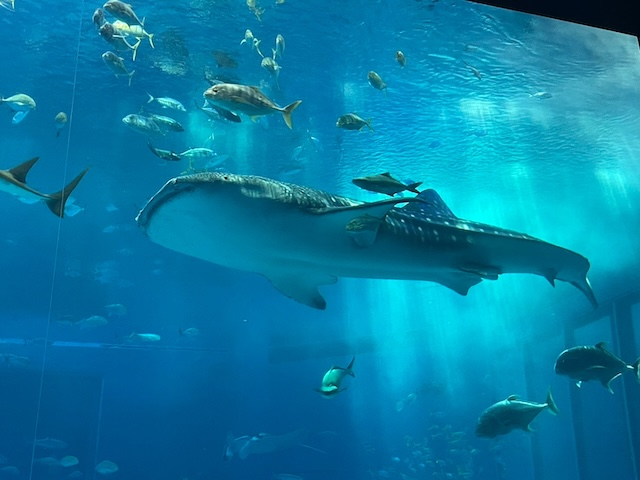
\includegraphics[width=\columnwidth]{sections/Nitta_Tokura/figure/zinbeizame.jpg}
  \end{minipage}
\end{figure}

\subsubsection*{・他にも...}
\begin{figure}[H]
  \begin{minipage}[b]{0.48\columnwidth}
    \centering
    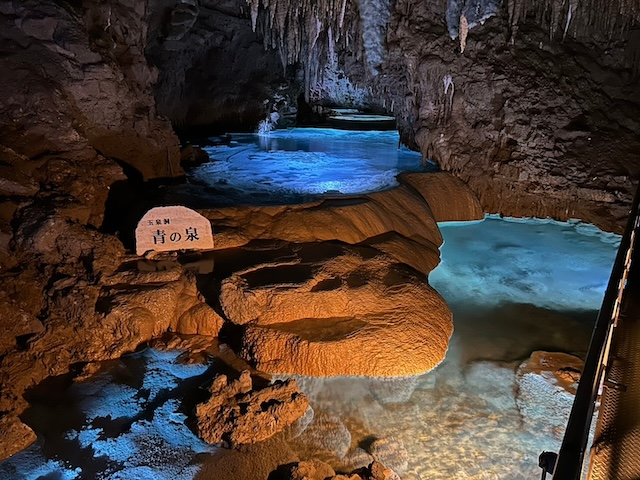
\includegraphics[width=\columnwidth]{sections/Nitta_Tokura/figure/tamasendou.jpg}
  \end{minipage}
  \hspace{0.04\columnwidth} % ここで隙間作成
  \begin{minipage}[b]{0.48\columnwidth}
    \caption{\\
    玉泉洞\\
    国内最大規模の鍾乳洞は圧巻で、特に青の泉はきれいにライトアップされていてきれいでした。
    }
  \end{minipage}
\end{figure}

部員全員が泊港に集合した後、高速船に乗り座間味島に向かいました。
\begin{figure}[H]
  \begin{minipage}[b]{0.48\columnwidth}
    \centering
    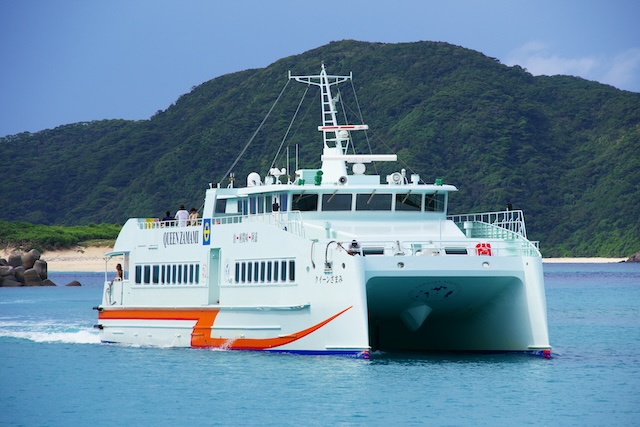
\includegraphics[width=\columnwidth]{sections/Nitta_Tokura/figure/queen_zamami.jpg}
  \end{minipage}
  \hspace{0.04\columnwidth} % ここで隙間作成
  \begin{minipage}[b]{0.48\columnwidth}
    \caption{\\
    乗船した高速船\\
    夕方には本島泊港を高速船「クイーンざまみ」で出発しました。高速船は時速約60 kmで航行する高速船で非常に揺れました。ただ、本島と座間味島をおよそ1時間でつなぐ速さには驚きました...!
    }
  \end{minipage}
\end{figure}

\begin{figure}[H]
  \begin{minipage}[b]{0.48\columnwidth}
    \caption{\\
    夕食のタコライス\\
    部員たちで夕食にタコライスと豚汁を作りました。とても美味しかったです!
    }
  \end{minipage}
  \hspace{0.04\columnwidth} % ここで隙間作成
  \begin{minipage}[b]{0.48\columnwidth}
    \centering
    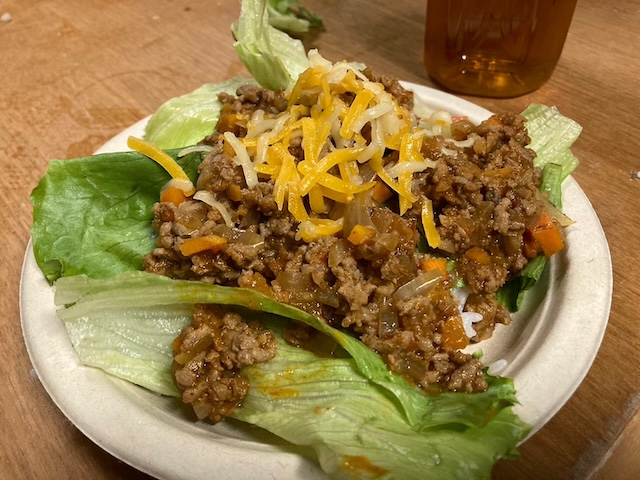
\includegraphics[width=\columnwidth]{sections/Nitta_Tokura/figure/takoraisu.JPG}
  \end{minipage}
\end{figure}

\subsection{3日目}
午前中、天候がとても良かったので、座間味島の美しい海で海水浴を楽しみました。
\begin{figure}[H]
  \begin{minipage}[b]{0.48\columnwidth}
    \centering
    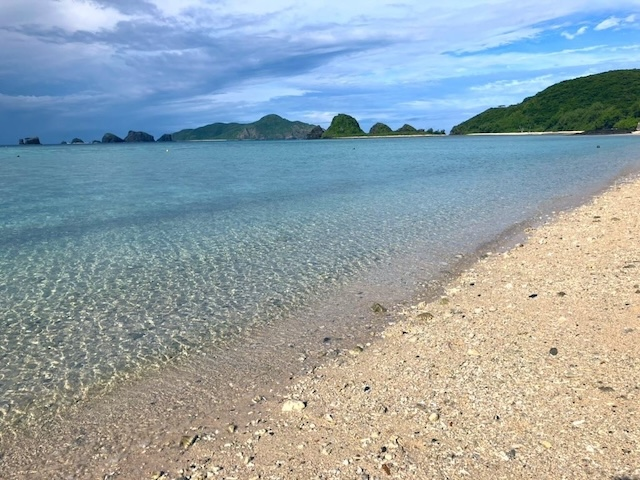
\includegraphics[width=\columnwidth]{sections/Nitta_Tokura/figure/tikaiumi.JPG}
  \end{minipage}
  \hspace{0.04\columnwidth} % ここで隙間作成
  \begin{minipage}[b]{0.48\columnwidth}
    \caption{\\
    座間味島の海\\
    島の海は驚くほど澄んでいて、浅瀬には色とりどりの魚たちが泳いでいるのが見えました。
    }
  \end{minipage}
\end{figure}

\begin{figure}[H]
  \begin{minipage}[b]{0.48\columnwidth}
    \caption{\\
    少し沖の海\\
    さらに沖の方へ進むと、さらに大きな魚が泳いでいるのを発見しました。コテージ近くのビーチは遠浅だったので沖に行っても間近でサンゴが見れました。
    }
  \end{minipage}
  \hspace{0.04\columnwidth} % ここで隙間作成
  \begin{minipage}[b]{0.48\columnwidth}
    \centering
    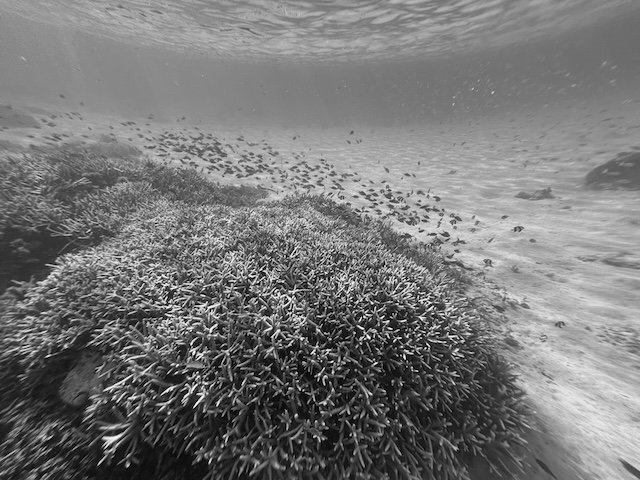
\includegraphics[width=\columnwidth]{sections/Nitta_Tokura/figure/okinoumi.jpg}
  \end{minipage}
\end{figure}

お昼にはみんなでバーベキューをする計画を立てていましたが、残念ながら天候が悪化し、雨が降ってしまいました。そのため、予定を変更し、屋外でのバーベキューは諦めて、コンロでお肉を焼いて食べました。
\begin{figure}[H]
  \begin{minipage}[b]{0.48\columnwidth}
    \centering
    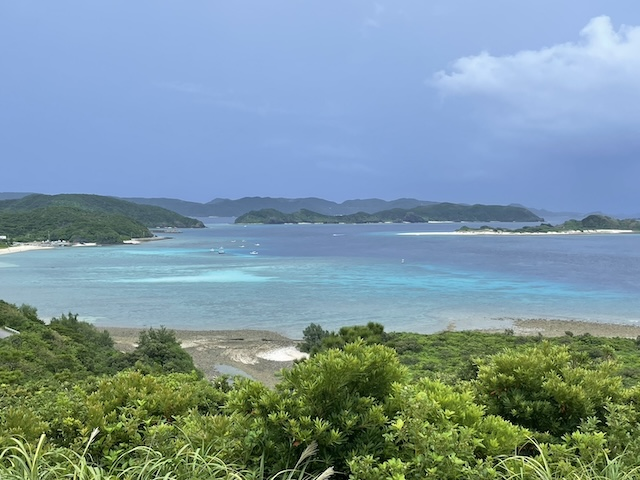
\includegraphics[width=\columnwidth]{sections/Nitta_Tokura/figure/tenboudaikaranonagame.jpg}
  \end{minipage}
  \hspace{0.04\columnwidth} % ここで隙間作成
  \begin{minipage}[b]{0.48\columnwidth}
    \caption{\\
    展望台からの眺め\\
    夜に行う天体観測に備えて、一部の人は星空がよく見える展望台を探しに行きました。展望台からは、青く広がる海が一望でき、その景色は息をのむほど素晴らしかったです!
    }
  \end{minipage}
\end{figure}

\begin{figure}[H]
  \begin{minipage}[b]{0.48\columnwidth}
    \caption{\\
    夕食で出てきたフ―チャンプル\\
    港近くのお店で夕食を食べました。沖縄の郷土料理でとてもおいしかったです。
    }
  \end{minipage}
  \hspace{0.04\columnwidth} % ここで隙間作成
  \begin{minipage}[b]{0.48\columnwidth}
    \centering
    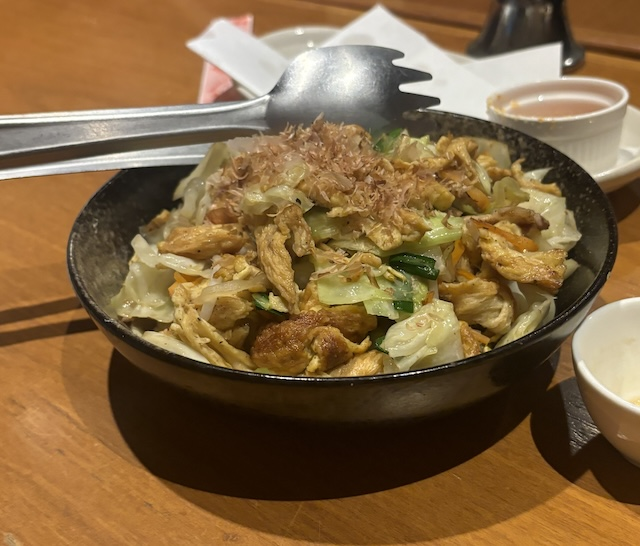
\includegraphics[width=0.8\columnwidth]{sections/Nitta_Tokura/figure/hu-tyanpuru.jpg}
  \end{minipage}
\end{figure}

展望台組と海岸組に分かれてそれぞれの場所で天体観測をしました。残念ながら、夜の天気もあまり良くなく、雲が広がっていましたが、時折雲の隙間から見える星々を楽しむことができました。海岸では砂浜に横たわって眺めた夜空は、昼間とはまた違った趣があり、まるで星々が手に届きそうなほど美しく感じました。
\begin{figure}[H]
  \begin{minipage}[b]{0.48\columnwidth}
    \centering
    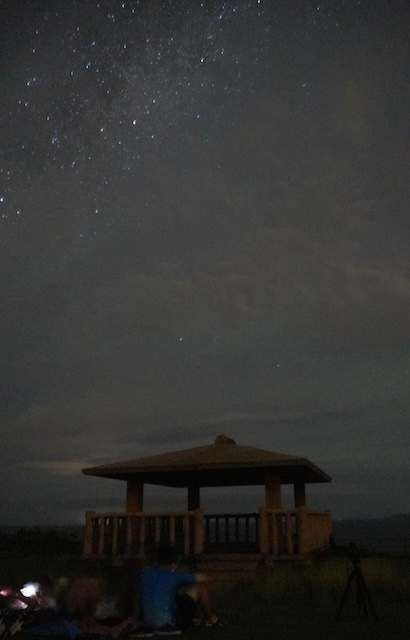
\includegraphics[width=0.8\columnwidth]{sections/Nitta_Tokura/figure/3nitimeyoru.jpg}
  \end{minipage}
  \hspace{0.04\columnwidth} % ここで隙間作成
  \begin{minipage}[b]{0.48\columnwidth}
    \caption{\\
    天体観測\\
    少し曇りがかった夜空で、星々が淡く瞬き、静かな癒しを感じました。
    }
  \end{minipage}
\end{figure}

\subsubsection*{・座間味島の様子}
\begin{figure}[H]
  \begin{minipage}[b]{0.48\columnwidth}
    \centering
    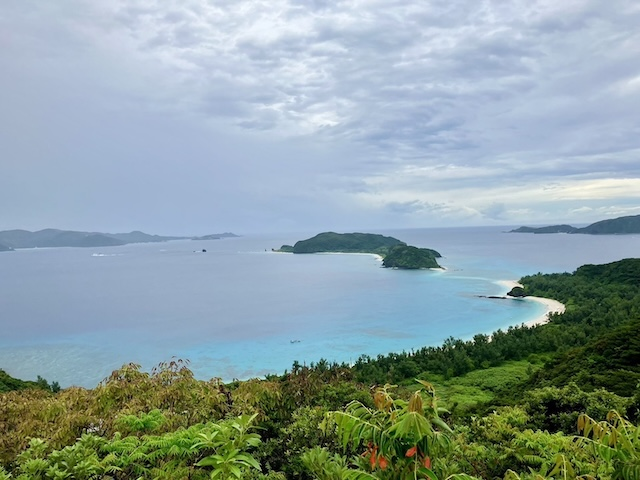
\includegraphics[width=0.85\columnwidth]{sections/Nitta_Tokura/figure/zamamiumi.jpg}
  \end{minipage}
  \hspace{0.04\columnwidth} % ここで隙間作成
  \begin{minipage}[b]{0.48\columnwidth}
    \caption{\\
    座間味島の海\\
    本島と比べて透明度が圧倒的に高く、またウミガメなども見れます!
    }
  \end{minipage}
\end{figure}

\begin{figure}[H]
  \begin{minipage}[b]{0.48\columnwidth}
    \caption{\\
    建物に置いてあったシーサー\\
    シーサーには狛犬のような魔除けの意味を持ち、沖縄では屋根の上や玄関に置かれています。観光客のお土産としても人気です。
    }
  \end{minipage}
  \hspace{0.04\columnwidth} % ここで隙間作成
  \begin{minipage}[b]{0.48\columnwidth}
    \centering
    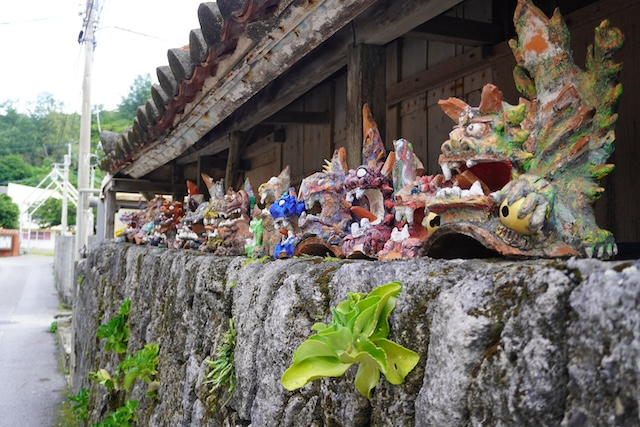
\includegraphics[width=\columnwidth]{sections/Nitta_Tokura/figure/zamami_si-sa-.jpg}
  \end{minipage}
\end{figure}

\begin{figure}[H]
  \begin{minipage}[b]{0.48\columnwidth}
    \centering
    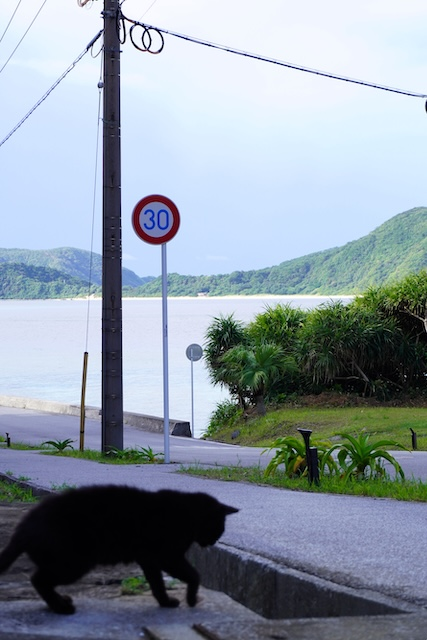
\includegraphics[width=0.8\columnwidth]{sections/Nitta_Tokura/figure/zamami_neko.jpg}
  \end{minipage}
  \hspace{0.04\columnwidth} % ここで隙間作成
  \begin{minipage}[b]{0.48\columnwidth}
    \caption{\\
    島にいた猫\\
    島には多く猫がいました。近くの別の島では鹿もいました。
    }
  \end{minipage}
\end{figure}

\subsection{4日目}

\begin{figure}[H]
  \begin{minipage}[b]{0.48\columnwidth}
    \centering
    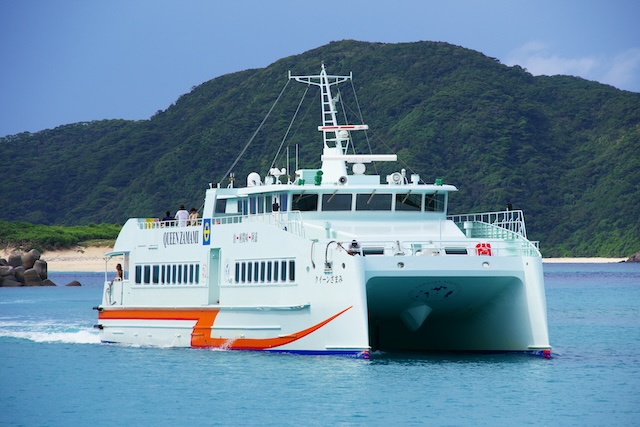
\includegraphics[width=\columnwidth]{sections/Nitta_Tokura/figure/queen_zamami.jpg}
  \end{minipage}
  \hspace{0.04\columnwidth} % ここで隙間作成
  \begin{minipage}[b]{0.48\columnwidth}
    \caption{\\
    2回目の高速船\\
    高速船で沖縄本島へと移動しました。台風が近づいている影響で少し海が荒れ、船は大きく揺れましたが、甲板に上がると爽やかな潮風が肌に心地よかったです。
    }
  \end{minipage}
\end{figure}
沖縄本島に到着後は、各自が自由に過ごす時間となりました。私は国際通りを散策し、料理を楽しんだり、お土産を買うためにお店をいくつも巡りました。
\begin{figure}[H]
  \begin{minipage}[b]{0.48\columnwidth}
    \caption{\\
    昼食で食べたA$\&$W\\
    沖縄で有名なハンバーガーチェーン店。独特な味のルートピアやカーリーフライという、らせん状のポテトが人気です。
    }
  \end{minipage}
  \hspace{0.04\columnwidth} % ここで隙間作成
  \begin{minipage}[b]{0.48\columnwidth}
    \centering
    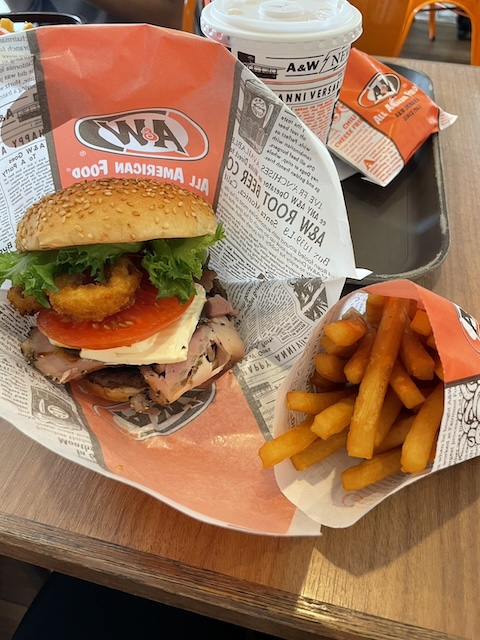
\includegraphics[width=0.7\columnwidth]{sections/Nitta_Tokura/figure/aandw.jpg}
  \end{minipage}
\end{figure}

活気ある通りの雰囲気に包まれながら、最後のひとときを満喫しました。\\
その後、飛行機で成田空港へと向かい、窓の外には美しい夕焼けが広がっていました。
\begin{figure}[H]
  \begin{minipage}[c]{0.49\textwidth}
  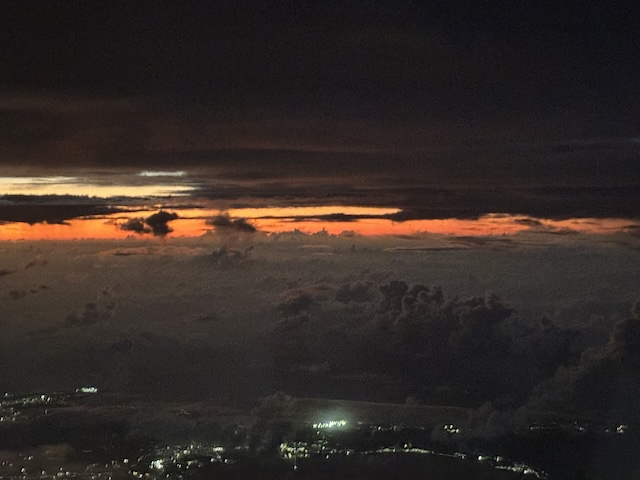
\includegraphics[width=\columnwidth]{sections/Nitta_Tokura/figure/yuuyake.jpeg}
  \end{minipage}
  \hspace{0.04\columnwidth} % ここで隙間作成
  \begin{minipage}[c]{0.4\textwidth}
    \caption{\\
    飛行機から見えた夕焼け\\
    合宿の最後にふさわしいきれいな夕焼けでした。
    }
  \end{minipage}
\end{figure}
\section{最後に}
\begin{figure}[H]
  \centering
  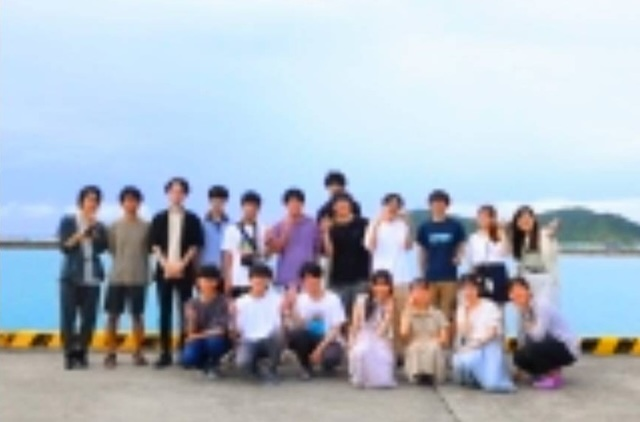
\includegraphics[width=10cm]{sections/Nitta_Tokura/figure/syuugousyasinn.JPG}
  \caption{集合写真}
\end{figure}
今回の天文部の合宿は、天候にはあまり恵まれなかったものの、仲間たちとの交流を深め、さまざまな楽しい経験を共有できたことで、忘れられない素晴らしい旅となりました。

\end{document}


\end{document}
